\chapter{Implementación}

En este capítulo se comenta cómo el diseño fue llevado a la práctica.
Empezaremos explicando la integración el servicio de localización, a continuación la implementación del servicio de \textit{Backend}, y por último, el  desarrollo de la aplicación móvil.

% Servicio de localización
\section{Servicio de localización}
Para integrar los servicios de \textit{Situm} en una aplicación \textit{iOS} hay que seguir los siguientes pasos \cite{noauthor_situm_nodate}.

\begin{enumerate}
\item \textbf{Crear una cuenta de \textit{Situm Dashboard}.} Así podremos empezar a subir planos de edificios y calibraciones \cite{noauthor_situm_nodate} a nuestro perfil. 

\item \textbf{Subir planos de un edificio.}\label{item:calib~.aciones} Hay que subir los planos de cada planta. Se debe situar el plano correctamente sobre un mapa de \textit{Google}. Una vez subido el primero, los siguientes se situarán sobre el mapa de la misma manera: mismas coordenadas, altura y orientación. Por eso es importante que todos los planos correspondientes a las plantas de un mismo edificio tengan la misma resolución y estén alineados, ver figura~\ref{fig:planos-situm}.

\item{}\textbf{Subir las calibraciones.} Para ello se utilizó la aplicación \textit{Android} que hay disponible en la \textit{Play Store} \cite{noauthor_aplicacion_nodate}. Iniciando sesión con la misma cuenta del \textit{Dashboard} se ``calibra'' el edificio, es decir, moverse por el edificio indicando y, a medida que se avanza, identificar en el mapa que muestra la aplicación cual es nuestra posición.

\item{}\textbf{Añadir las librerías de \textit{Situm} a nuestra aplicación.} Debemos descargar el \textit{framework} \cite{situm_situm_nodate} e incorporarlo a nuestro proyecto de \textit{Xcode}, ver figura~\ref{fig:sdk-xcode}.

\item{}\textbf{Añadir la \textit{API KEY} al proyecto y empezar a trabajar.} Hay tutoriales oficiales de \textit{Situm} sobre como añadir la \textit{API KEY} y empezar a obtener la información sobre los edificios que hay subidos en la cuenta del \textit{Dashboard} \cite{noauthor_situm_nodate}, ver figura~\ref{fig:api-situm-code}.

\begin{figure}[tbp]
\centering
\subfigure{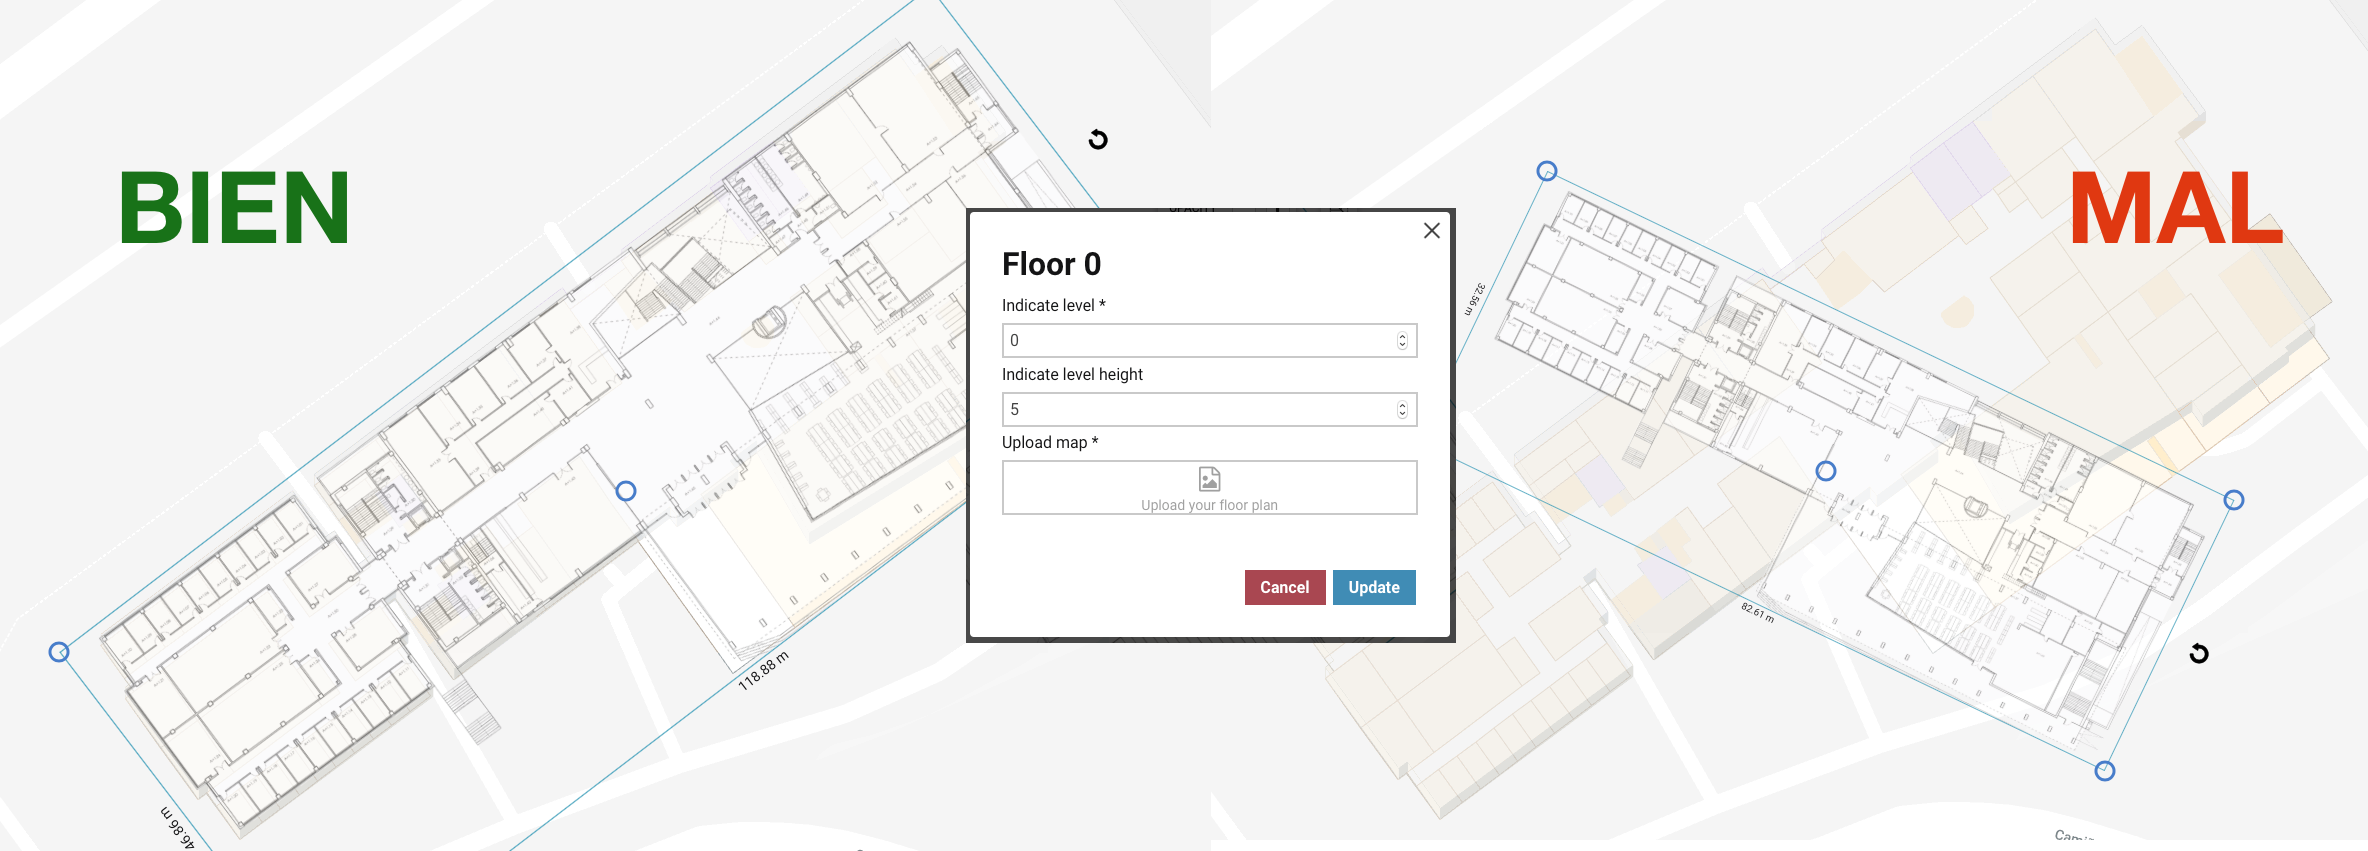
\includegraphics[width=\textwidth]{figures/planos-situm.png}\label{fig:planos-situm}}
\vspace{3ex}
\subfigure{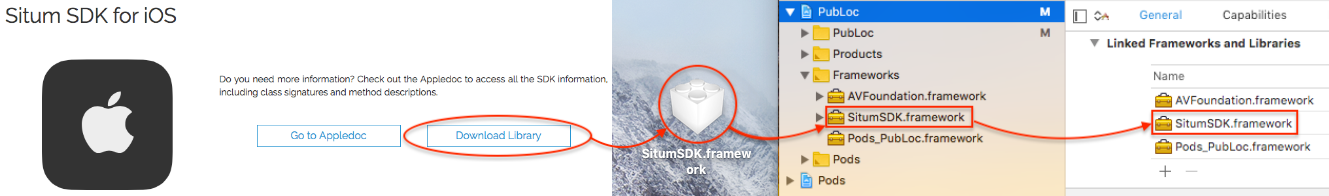
\includegraphics[width=\textwidth]{figures/sdk-xcode.png}\label{fig:api-situm-code}}
\vspace{3ex}
\subfigure{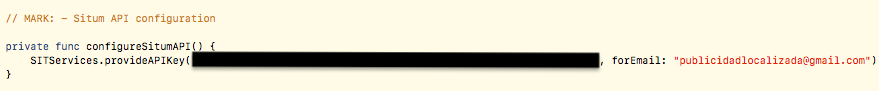
\includegraphics[width=\textwidth]{figures/api-situm-code.png}\label{fig:sdk-xcode}}
\caption[Configuración de la localización de \textit{Situm}.]{Configuración de la localización de \textit{Situm}: (arriba) subir los planos alineado de cada planta; (centro) recoger el \textit{API KEY} en el \textit{Dashboard} y descarga en el directorio de \textit{frameworks} del proyecto; y (abajo) añadir a \textit{Linked Frameworks and Libraries}.}
\end{figure}
\end{enumerate}

\subsection{Simulación con fichero \textit{JSON}}
Para hacer pruebas con la aplicación se decidió utilizar un fichero \textit{JSON}, como se explica en el apartado~\ref{sec:simul_subsec}. El contenido de este fichero es una lista de objetos \textit{JSON} y cada uno de ellos contendría unas coordenadas (longitud y latitud) y la planta del edificio en la que estaría ubicado (ver código \ref{list:json-simul}).

Desde la aplicación, se recorre el fichero en bucle y se va moviendo una chincheta sobre el mapa, saltando de un punto a otro y cambiando de planta cuando sea necesario.
Hay que señalar que se debe animar el movimiento para que no se aprecien los saltos de manera brusca.
El resultado final es idéntico al que veríamos en cualquier aplicación de mapas.

Para crear este fichero usamos una herramienta \textit{online} \cite{noauthor_herramienta_nodate} que genera un \textit{JSON} a partir de una ruta que nosotros mismos diseñamos marcando una sucesión de puntos en un mapa (figura~\ref{fig:sim-json-gen}). Pero la información sobre el piso hubo que metérsela a mano.

\begin{figure}[bt]
\centering
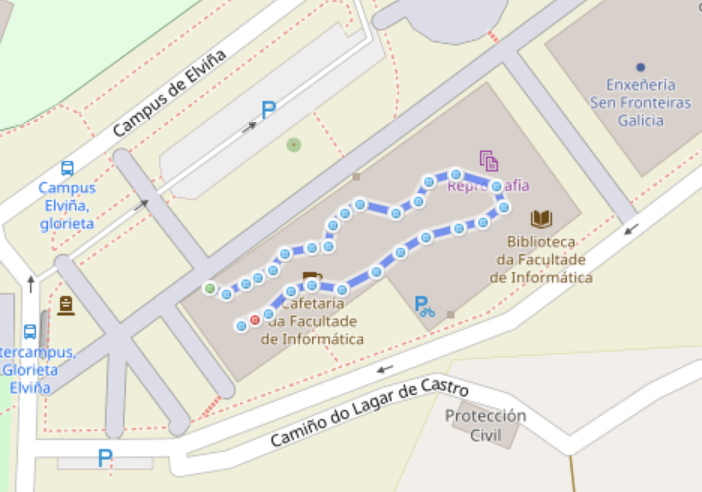
\includegraphics[width=0.6\textwidth]{figures/sim-json-gen.png}
\caption{Creación de ruta exportables a \textit{JSON}.\label{fig:sim-json-gen}}
\end{figure}

\begin{lstlisting}[language=json,style=interfaces,caption={Fragmento de simulación \textit{JSON}, coincide con el cambio del piso 0 al 1.},label={list:json-simul}]
...
{
   "lon": -8.41110706,
   "lat": 43.3329964,
   "lev": 0
}, {
   "lon": -8.41106414,
   "lat": 43.332969,
   "lev": 0
}, {
   "lon": -8.41105341,
   "lat": 43.3329222,
   "lev": 1
}
...
\end{lstlisting}


% Servicio de Backend
\section{Servicio de \textit{Backend}}
En esta sección se comenta  el desarrollo de toda la parte de servidor o \textit{Backend} del proyecto. Empezaremos por la fase de autenticación, la \textit{API REST}, el uso de las \textit{Cloud Functions} y la implementación del modelo de datos.

\subsection{Autenticación}
Cuando un usuario se autentica en la aplicación mediante cualquiera de los métodos ofrecidos por \textit{Firebase}, se le asigna un determinado \textit{token} de usuario, ver figura~\ref{fig:access-token}.

\begin{figure}[bt]
\centering
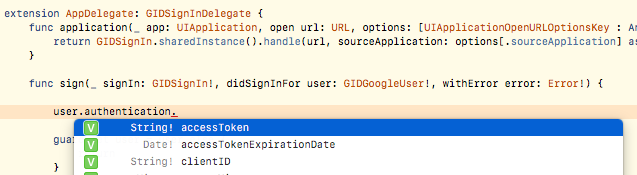
\includegraphics[width=0.8\textwidth]{figures/access-token.png}
\caption{El \textit{token} es un \textit{string} que se puede obtener tras una autenticación exitosa.\label{fig:access-token}}
\end{figure}

Lo único que hay que hacer es añadir ese \textit{token} como una \textit{query-string} a toda \textit{URL} a la que hagamos una petición.

\subsection{\textit{API REST}}
Para comunicarnos a la \textit{API REST} se utilizó la librería \textit{Alamofire} \cite{noauthor_alamofire_nodate}, la cual permite realizar de manera sencilla peticiones \textit{HTTP}. A continuación, hablaremos sobre como se implementó esta importante parte del proyecto.

\subsubsection*{Composición de las \textit{URLs}} \label{comp:url}
Dada la estructura en árbol de una base de datos no relacional, para formar la \textit{URL} hay que ir concatenando al identificador del proyecto las claves de aquellos nodos por los que hay que pasar para llegar al que nos interesa (separados por ``\textit{/}''). Cuando se llega al nodo al que se quiere hacer la petición, se debe concatenar ``\textit{.json}'' a la \textit{URL}. Por ejemplo la \textit{URL} del nodo de la figura~\ref{fig:node} sería: \url{https://publoc-1234.firebaseio.com/Buildings/3598/Shops/-LKnOeINwIY7m0wEfK90/Offers/-LKnSVU1KGgrAuRQymv7.json}

\subsubsection*{Peticiones}
A continuación, se comentan los cuatro tipos de peticiones que se utilizaron.

\paragraph{\textit{GET}.} Petición utilizada para obtener información sobre un nodo de la base de datos. El resultado de la petición es una cadena de texto en formato \textit{JSON} que representa al nodo y cuyos campos se deben \textit{mapear} a un objeto para poder trabajar con él en la aplicación. La \textit{URL} deberá representar al nodo deseado, ver sección~\ref{comp:url}.

\paragraph{\textit{POST}.} Petición utilizada para crear un nuevo nodo en la base de datos. Cuando hacemos una petición de este tipo, debemos enviarle una cadena de texto en formato \textit{JSON} que represente el valor del nodo que queremos crear en el cuerpo de la petición. La respuesta que nos devuelve el servidor es una cadena de texto en formato \textit{JSON} que contiene el identificador del nodo que se acaba de crear. La \textit{URL} deberá representar al nodo en el que se desea insertar al nuevo, ver sección~\ref{comp:url}.

\paragraph{\textit{PATCH}.} petición utilizada para modificar el contenido de un nodo en la base de datos. Cuando hacemos una petición de este tipo, debemos enviarle una cadena de texto en formato \textit{JSON} que represente aquellos campos del nodo que queremos modificar, como cuerpo de la petición. La respuesta que nos llega de servidor es una cadena de texto en formato \textit{JSON} que contiene aquellos campos del nodo que han sido modificados. La \textit{URL} deberá representar al nodo que se quiere modificar, ver sección~\ref{comp:url}.

\paragraph{\textit{REMOVE}.} petición utilizada para eliminar un nodo. Esta petición devuelve simplemente \textit{200 OK} si se realiza correctamente. La \textit{URL} deberá representar al nodo que se quiere borrar.

\subsubsection*{\textit{Stream} de un nodo}

\begin{lstlisting}[style=interfaces,caption=Fragmento de código correspondiente a un \textit{streaming}.,label={list:alamo-stream}]
public static func stream(url: String, completionFailure: @escaping (DataResponse<Any>) -> Void, completionStream: @escaping (Data) -> Void) -> Request {
	return Alamofire.request(url, method: .get, parameters: nil, encoding: JSONEncoding.default, headers: ["Accept": "text/event-stream"]).responseJSON { (response) in
		switch response.result {
		case .success:
			break
		case .failure:
			completionFailure(response)
		}
	}.stream { (data) in
		completionStream(data)
	}
}
\end{lstlisting}

Desde el controlador se puede hacer \textit{streaming} a un nodo de la base de datos para modificar la vista si se produce un cambio en este, haciendo un petición \textit{GET} a un nodo con la cabecera \textbf{``\textit{Accept}''} a \textbf{``\textit{text/event-stream}''}. La librería \textit{Alamofire} facilita esta tarea, ver fragmento de código~\ref{list:alamo-stream}.


\subsection{\textit{Cloud Functions}}
Como se decidió tarde incluir esta tecnología al proyecto, se utilizaron muchas menos \textit{Cloud Functions} de las que se deberían. Si se hubiesen utilizado desde el principio, muchas tareas podrían haberse realizado de una manera más simple. A continuación un par de ejemplos en los que si se usaron este tipo de funciones, de los dos tipos comentados en el apartado  \ref{sec:cloud_functions}.

\subsubsection*{\textit{Cloud functions} activadas por peticiones \textit{HTTP}}
\begin{lstlisting}[style=interfaces,caption=\textit{Cloud Function} activada por petición \textit{HTTP}.,label={list:cloud-http}]
exports.removeOldOffers = functions.https.onRequest((req, res) => {
const timeNow = Date.now();
	const messagesRef = admin.database().ref('/Buildings');
	messagesRef.once('value', (snapshot) => {
		snapshot.forEach((child) => {
			child.ref.child('/Shops').once('value', (snapshot) => {
				snapshot.forEach((child) => {
					child.ref.child('/Offers').once('value', (snapshot) => {
						snapshot.forEach((child) => {
							if (Number(child.val()['expiration']) <= timeNow) {
								child.ref.set(null);
							}
						});
					});
				});
			});
		});
	});
	return res.status(200).end();
});
\end{lstlisting}

Se creó una función que repasa todos los nodos de ofertas, comprobando si alguna ha caducado. Esta función se activa mediante una petición \textit{HTTP} (ver fragmento de código~\ref{list:cloud-http}), como de momento \textit{Google} no permite programar peticiones periódicas, hubo que utilizar un servicio externo.

\begin{lstlisting}[style=interfaces,language=bash,label={list:watch},caption=Comando que ejecuta una petición \textit{HTTP} correspondiente a una \textit{Cloud Function} cada diez segundos.]
watch -n10 curl -X GET https://us-central1-publoc-1234.cloudfunctions.net/removeOldOffers
\end{lstlisting}

Se decidió ejecutar un comando en terminal que hace la petición cada diez segundos (ver comando \ref{list:watch}), limpiando así las ofertas caducadas. No se hace con más frecuencia, porque superaríamos la tasa de peticiones por unidad de tiempo que permite \textit{Firebase}.


\subsubsection*{\textit{Cloud functions} activadas tras cambios en la base de datos}
Se creó una función que detecta un escaneo en una oferta, entonces resta una unidad al campo de ese mismo nodo que contiene el número de ofertas restantes y si este llega a cero, la elimina.

\subsubsection*{Como incorporar las \textit{Cloud Functions} al proyecto}
Hay documentación oficial de \textit{Google} para dar nuestros primeros pasos con \textit{Cloud Functions} \cite{noauthor_documentacion_nodate}.

\begin{enumerate}
\item Lo primero que se necesita es un entorno \textit{Node.js} que servirá para escribir las funciones y \textit{Firebase CLI} que será lo que permita subir las funciones a \textit{Firebase}.

\item Una vez instalado \textit{Firebase CLI}, deberemos autenticarnos e inicializar el \textit{SDK} de \textit{Firebase} para \textit{Cloud Functions}. Escogeremos el lenguaje a utilizar para desarrollar las funciones, y nos creará la estructura de directorios necesaria en nuestro ordenador.

\item Ya podemos empezar a escribir nuestras funciones. Hay muchos códigos de ejemplo subidos por \textit{Google} \cite{noauthor_cloud_nodate-1}.

\item Una vez terminado el código, debe subirse a \textit{Firebase}, ver figura \ref{fig:cloud-deploy}.

\begin{figure}[tb]
\centering
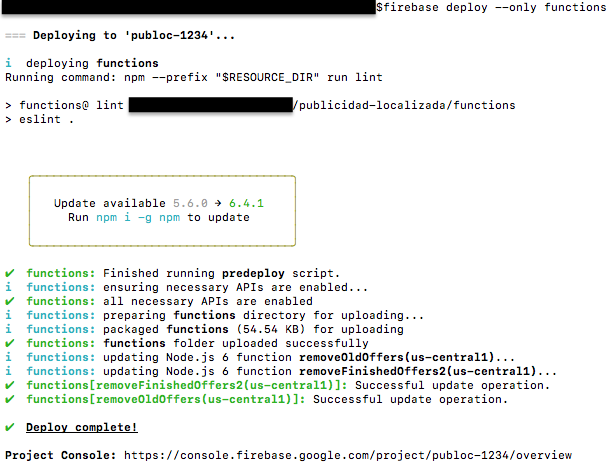
\includegraphics[scale=0.6]{figures/cloud-deploy.png}
\caption{Compilación y subida de funciones a \textit{Firebase}.\label{fig:cloud-deploy}}
\end{figure}
\end{enumerate}

\subsection{Modelo de datos}
Hay que tener en cuenta que no se trabaja con una base de datos que pueda seguir un modelo entidad relación. Por lo tanto, hay que seguir unas pautas a la hora de diseñar la estructura de los datos para un modelo de este tipo.

\subsubsection*{Evitar replicar nodos}
Para solventar el problema comentado en la sección anterior \ref{nosql}, habría que almacenar el identificador unívoco de un nodo dentro de otro para evitar replicar datos, es lo más parecido a una relación en un modelo relacional. Si hacemos esto, hay dos maneras de recuperar los datos.

\begin{enumerate}
\item\textbf{\textit{Firebase Database} + \textit{API REST}.} Lo malo es que nos vemos obligados a hacer dos peticiones o más para obtener todos los datos (depende del número de referencias a otros nodos). Esto incurre en un mayor tráfico de datos para el usuario, que lo notará en la factura, además de ralentizar las comunicaciones.

\item\textbf{\textit{Firebase Database} + \textit{Cloud Functions}.} Esta es la mejor de las soluciones, se hace una petición a una función y esta trabaja contra la base de datos, componiendo a nuestro gusta el \textit{JSON} que será devuelto.

No sólo nos ahorramos el tiempo y el coste de tener que hacer varias peticiones \textit{HTTP}, sino que también movemos al servidor la carga computacional de recolectar y juntar toda la información.
\end{enumerate}

\subsubsection*{Escalabilidad}
Es importante diseñar el modelo pensando en el futuro. Se deben estructurar los datos de manera que se pueda soportar a un gran número de usuarios. Por lo tanto, no se debe almacenar información de usuarios dentro de nodos que no son de usuarios, ver figura~\ref{fig:malaprac}. Por ejemplo, puede parecernos cómodo almacenar los identificadores de los usuarios que han escaneado una oferta dentro de la propia oferta. De esta manera, cuando un usuario pide una oferta, ya puede saber si la ha disfrutado sin necesidad de hacer otra petición para obtener sus ofertas disfrutadas.

\begin{figure}[tbp]
\centering
\subfigure{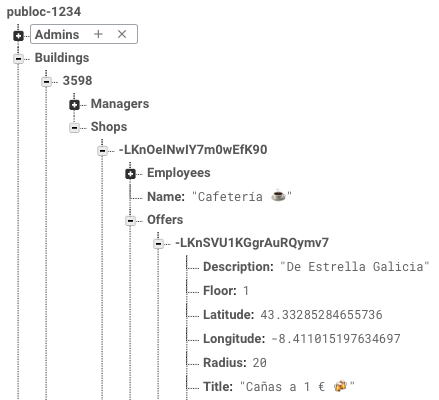
\includegraphics[width=0.65\textwidth]{figures/nodo-firebase.png}\label{fig:node}}
\vspace{3em}
\subfigure{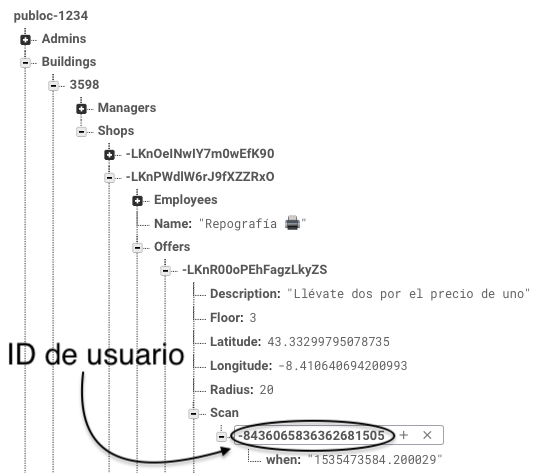
\includegraphics[width=0.65\textwidth]{figures/malaprac.png}\label{fig:malaprac}}
\caption{\textit{Firebase}: (a) Nodo de una oferta en la base de datos y (b) ejemplo de mala práctica en una estructura de datos no relacional, mezclando información de usuario con información general.}
\end{figure}

Esto funciona muy bien si la aplicación la usan cuatro personas, pero imaginemos un caso real de una aplicación con millones de usuarios que hiciera esto. En el caso de que \textit{YouTube} utilizara un modelo de datos no relacional y almacenara los \textit{likes} de usuarios en un vídeo con millones de reproducciones dentro del nodo del propio vídeo, cada vez que un usuario hiciera una petición a ese nodo, se descargaría también los datos de millones de usuarios.

Sin embargo, también se desperdician datos móviles, tiempo del usuario y memoria del dispositivo móvil. De ahí la importancia de separar los datos de usuario de los generales.

\section{Implementación de la aplicación móvil: MVC}
En esta sección se describen los procedimientos seguidos en el  desarrollo de la aplicación \textit{iOS}.
Más específicamente las capas de modelo, vista y  controlador.

\subsection{Modelo}
La implementación de la capa de modelo en una aplicación \textit{iOS} se centra en la comunicación con la base de datos: las peticiones.

%\subsubsection*{Peticiones}
Como ya se ha comentado, se emplea la librería \textit{Alamofire} para realizar las peticiones \textit{HTTP}. Una característica del lenguaje \textit{Swift}, es que permite pasar funciones como parámetros a otras funciones. De este modo se pudieron aislar los métodos que hacían las peticiones del resto del código.
Simplemente se declaran en cada controlador las funciones que se deben ejecutar al terminar cada petición y se pasan a los métodos genéricos que se comunican con la \textit{API REST}, junto con la \textit{URL}.

\begin{figure}[p]
\centering
\subfigure{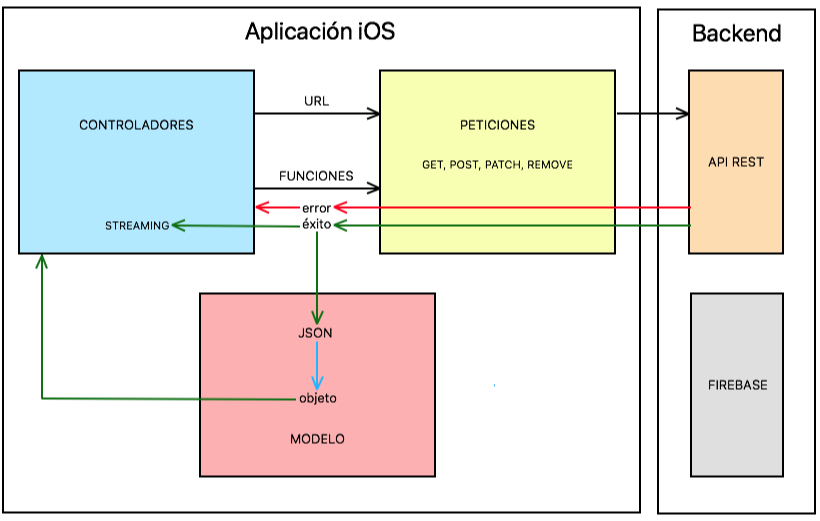
\includegraphics[width=0.89\textwidth]{figures/esquema-impl.png}\label{esquema-impl}}
\subfigure{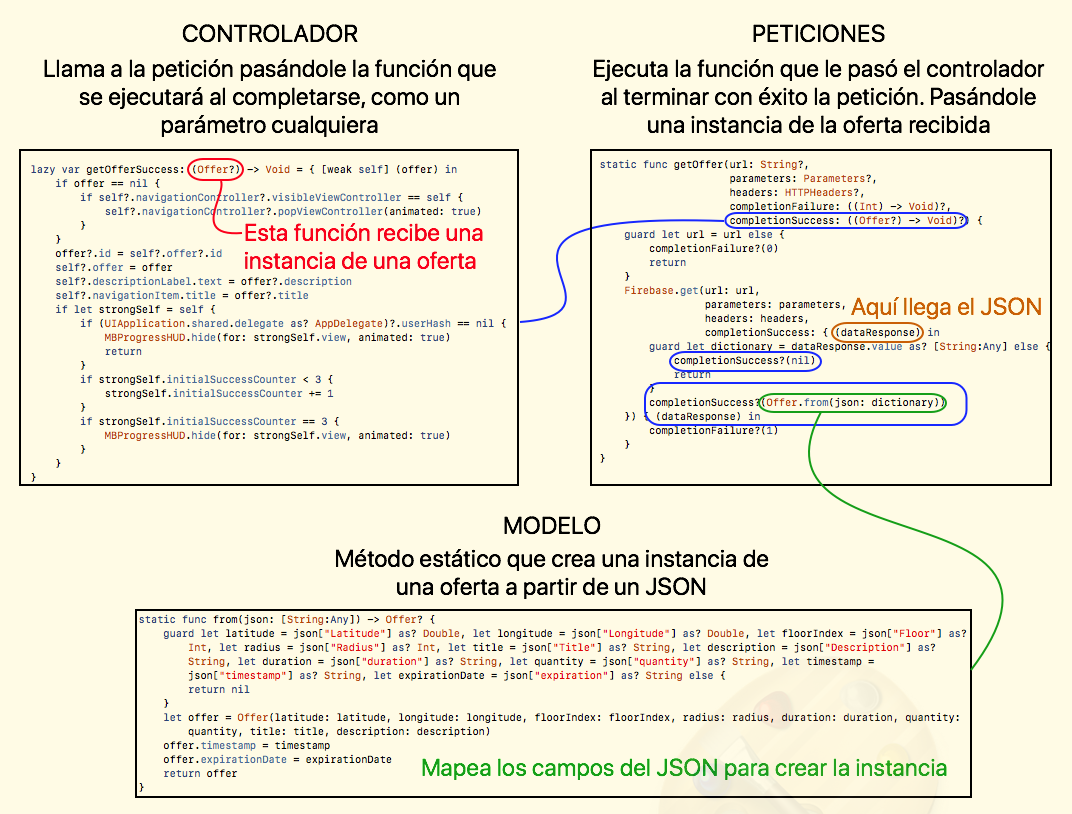
\includegraphics[width=\textwidth]{figures/ciclo.png}\label{fig:ciclo}}
\caption{MVC: (a) Comunicación de la aplicación \textit{iOS} con la \textit{API REST} y (b) funciones utilizadas en una petición.}
\end{figure}

Las peticiones se lanzan en segundo plano para no interrumpir a la aplicación.
Si se lanzasen en el \textit{thread} principal, la interfaz se quedaría bloqueada hasta que llegase la respuesta, y esto provocaría una mala experiencia de usuario. Cuando la respuesta llega, se ejecuta la función correspondiente según la respuesta obtenida, ver figura~\ref{esquema-impl}. Es recomendable mostrar un indicador de que se está cargando la información al realizar una petición, para después ocultarlo cuando la petición termina.

%\subsubsection*{Programación orientada a objetos}
Las peticiones nos devuelven una respuesta en formato \textit{JSON}, cuyos campos deben mapearse para crear instancias con las que poder trabajar. Estos métodos encargados de mapear los diccionarios \textit{JSON} funcionan como métodos constructores que devuelven una instancia que puede ser nula en caso de que no se mapeen correctamente los campos, véase la figura \ref{fig:ciclo}.

\subsection{Vista}
Antes de empezar con la implementación de la vista, se realizó un diseño con la herramienta \textit{Adobe Xd}, ver (figura~\ref{fig:adobe_xd}). Este programa es muy útil para elaborar las pantallas de la aplicación y ver como quedarían los colores, fuentes, dimensiones, etcétera; antes de ponerse a codificar. Ahorrando así mucho tiempo al programador que si no tuviese un prototipo tendría que compilar el proyecto y avanzar hasta la pantalla en cuestión para ver como quedaría cada vez que cambiase algo en la vista.

\begin{figure}[p]
\centering
\subfigure{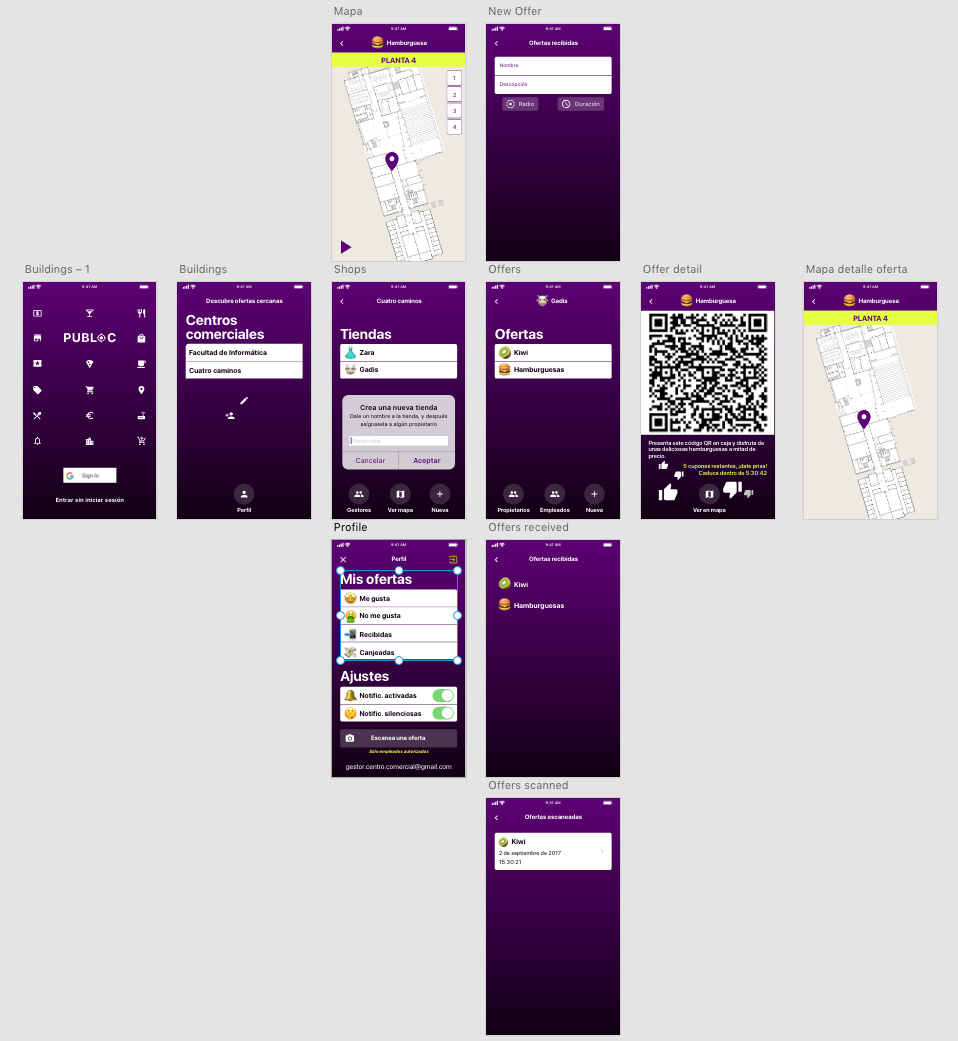
\includegraphics[width=0.85\textwidth]{figures/adobe_xd.png}\label{fig:adobe_xd}}
\subfigure{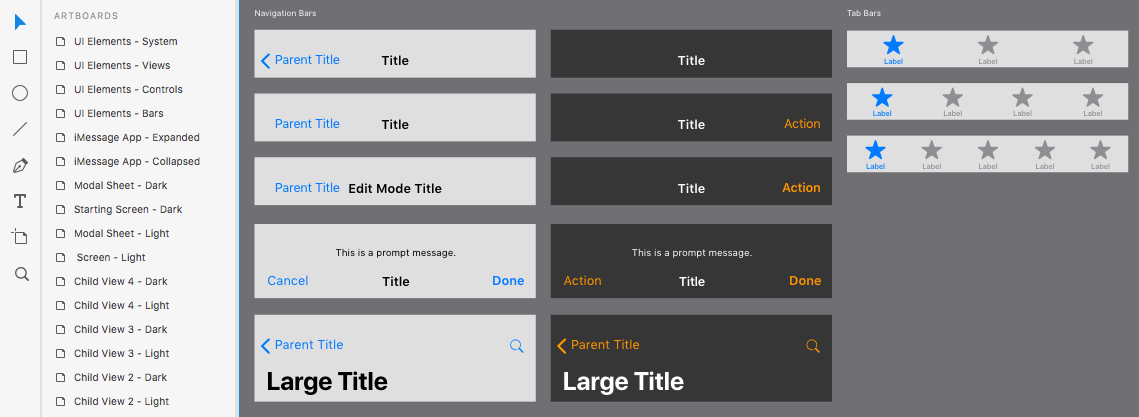
\includegraphics[width=0.89\textwidth]{figures/recursos-xd.png}\label{fig:recursos-xd}}
\caption{\textit{Adobe Xd}: (a) Captura de pantalla de la herramienta de diseño \textit{Adobe Xd} y (b) recursos oficiales de \textit{Apple}, importables para \textit{Adobe Xd}.}
\end{figure}

\textit{Adobe Xd} tiene plantillas de diversas resoluciones, que se corresponden con las resoluciones de los distintos dispositivos de \textit{Apple}, para realizar diseños sobre ellas. Además, desde la página oficial para desarrolladores de \textit{Apple} ofrecen recursos importables a \textit{Adobe Xd} \cite{noauthor_apple_nodate} como botones, cabeceras de tablas, etcétera. que cumplen con los principios de diseño recomendados para desarrollar aplicaciones \textit{iOS}, ver figura~\ref{fig:recursos-xd}.
Este programa también nos permite diseñar las transiciones entre pantallas y genera una simulación animada con la que podemos interactuar, como si de un emulador se tratase, ver figura~\ref{fig:simula-xd}.

\begin{figure}[tb]
\centering
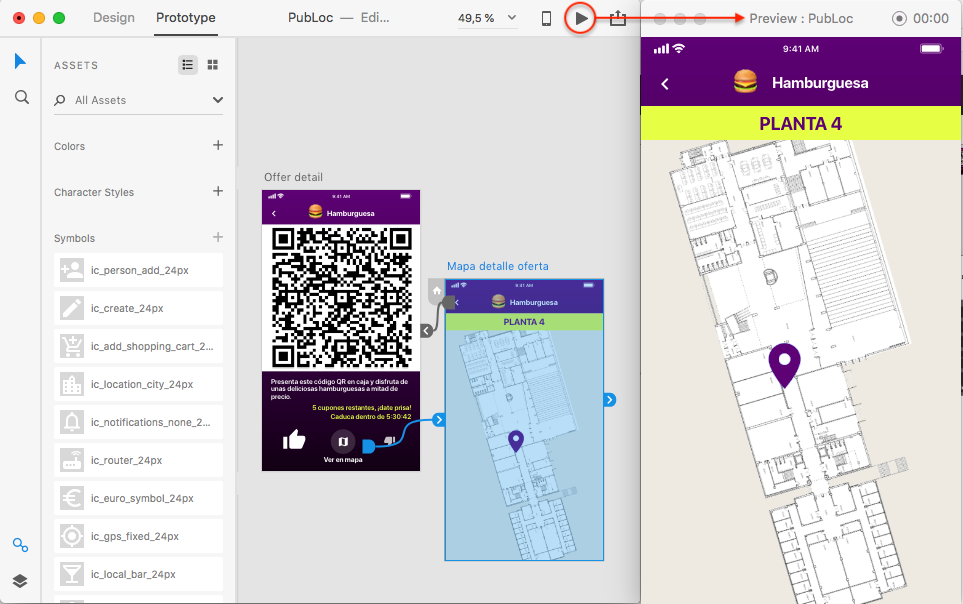
\includegraphics[scale=0.4]{figures/simulacion-xd.png}
\caption{Transiciones entre pantallas y simulación con \textit{Adobe Xd}.\label{fig:simula-xd}}
\end{figure}

\subsubsection*{Elección y disposición de los colores}
Primero se realizó una pequeña investigación sobre el efecto que producen los colores en las personas para saber que paleta de colores queríamos utilizar. Tras leer algún artículo \cite{noauthor_color_nodate} que hablaba sobre colores que atraen más a los hombres que a las mujeres, otros que se asocian a la comida, otros a los negocios o a la naturaleza, etcétera. Se decidió utilizar como color base el morado.

Una vez elegido el color base, hay que elegir unos colores que combinen con él de manera adecuada. Para ello conviene informarse sobre el círculo cromático y qué colores se relacionan entre sí (figura~\ref{fig:relacion-colores}).
Adobe ofrece una herramienta que facilita la elección de los colores \cite{noauthor_adobe_nodate}. A partir de un color base nos da los colores que combinarían con él (figura~\ref{fig:paleta-complementaria}).

\begin{figure}[tb]
\centering
\subfigure{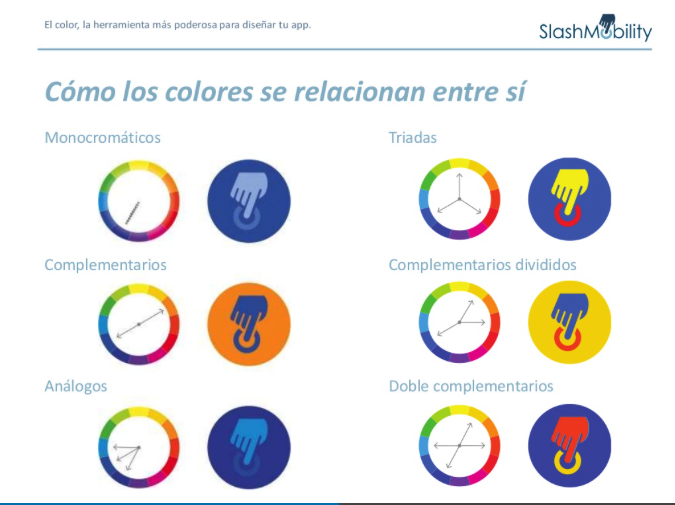
\includegraphics[width=0.48\linewidth]{figures/relacion-colores.png}\label{fig:relacion-colores}}
\subfigure{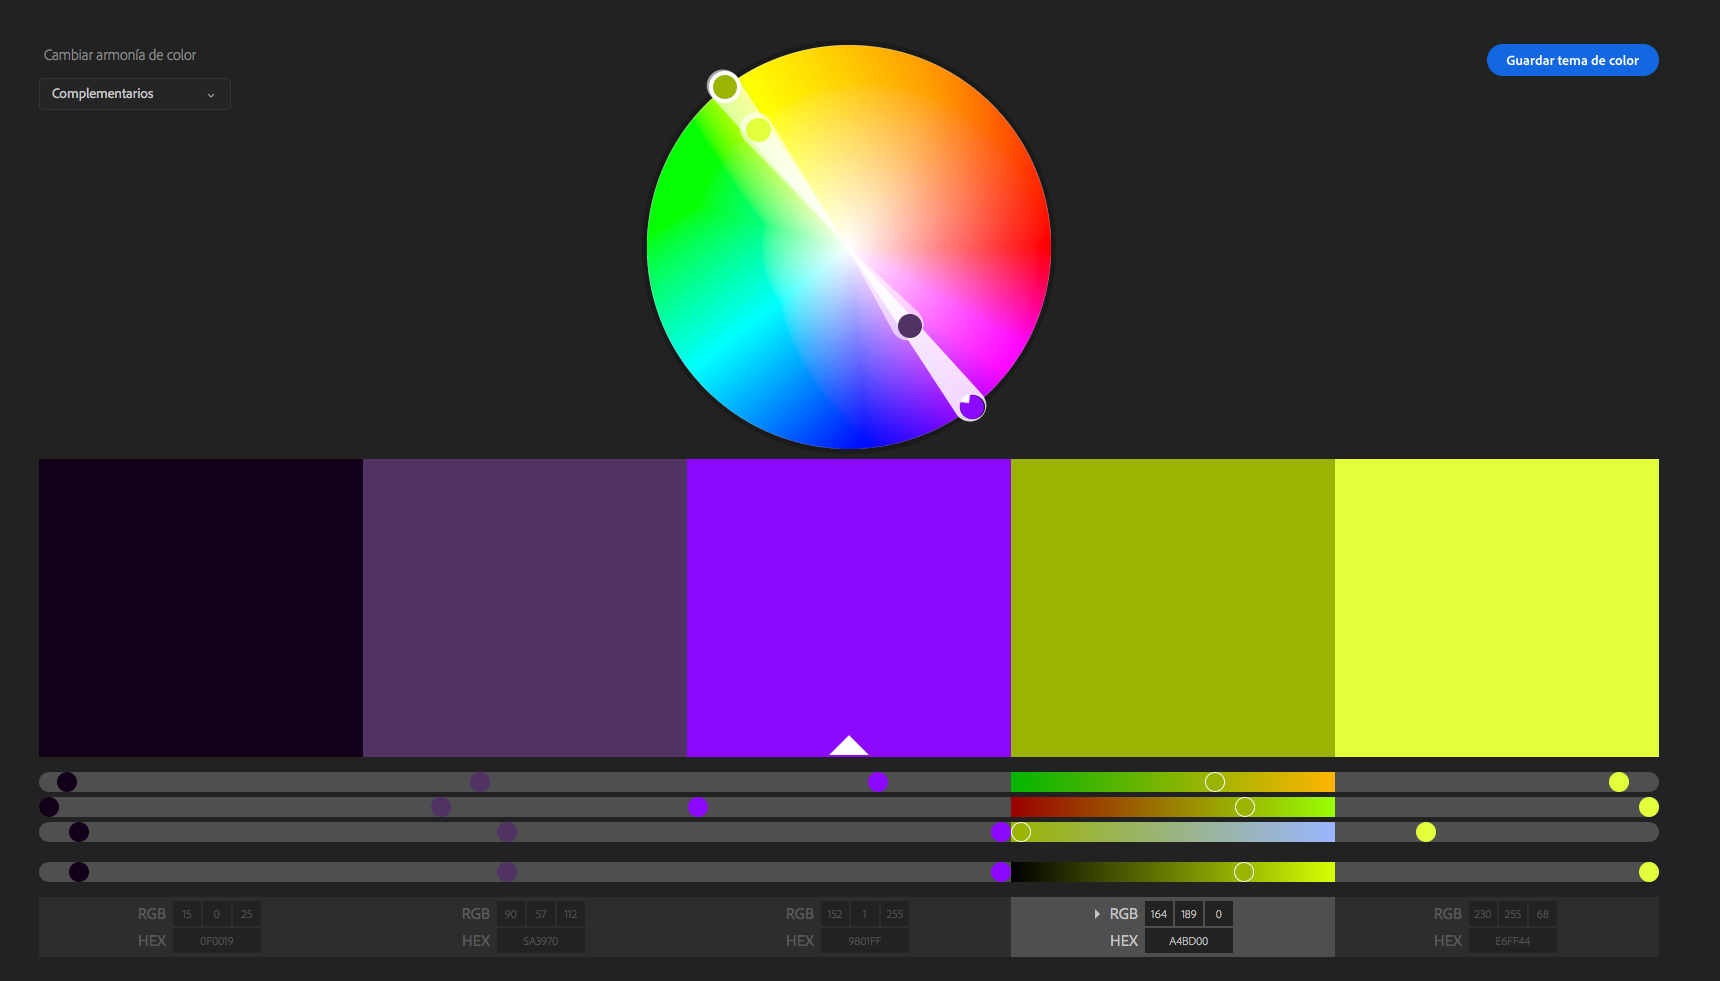
\includegraphics[width=0.48\linewidth]{figures/paleta-complementaria.png}\label{fig:paleta-complementaria}}
\caption{Arquitectura de colores: (a) Como combinar colores usando el círculo cromático y (b) paleta de colores utilizada, el morado y sus complementarios.}
\end{figure}


\subsubsection*{Implementación de la vista con \textit{Xcode}}
Una vez terminado el diseño, debemos incorporarlo a nuestra aplicación. Como se comentó en el capítulo \ref{planificacion_chap}, la implementación de la interfaz de usuario se dejó para el último \textit{sprint}, ya que al trabajar con una metodología \textit{SCRUM}, pueden surgir nuevas funcionalidades a medida que se avanza en el desarrollo. Esto puede tener su repercusión en la vista, siendo necesario añadir nuevos botones, tablas, mapas, etc.

\begin{figure}[tbp]
\centering
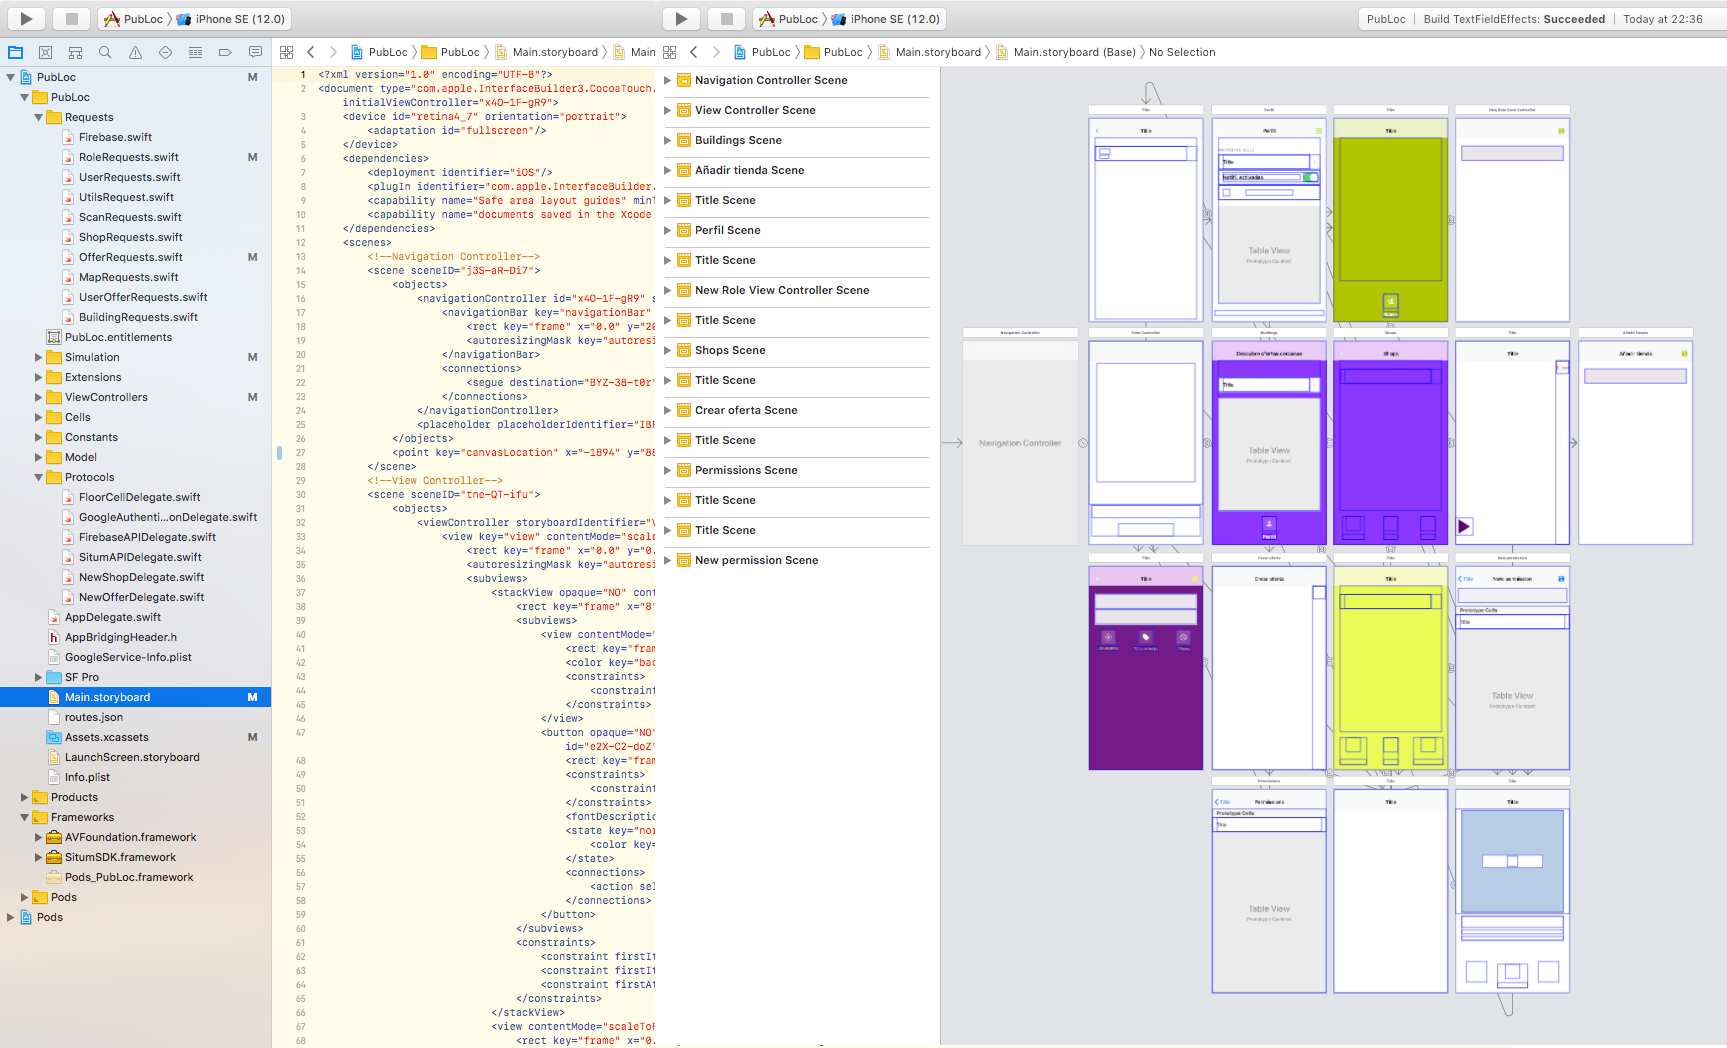
\includegraphics[scale=0.2]{figures/story-xml.png}
\caption{\textit{Interface Builder} vs \textit{xml}.\label{fig:story-xml}}
\end{figure}

El programa \textit{Xcode} permite desarrollar la vista de manera gráfica, esto facilita enormemente la tarea porque si no, habría que escribirlo todo en código \textit{xml} (figura~\ref{fig:story-xml}).
Aunque también se pueden implementar los elementos de la vista programáticamente, es decir, creándolos desde el controlador con \textit{Swift}. Este método tiene ventajas, como el hecho de tener todo en un mismo sitio bien organizado, muchas veces en el \textit{Interface Builder} se toca algo que está un poco escondido y luego pasan cosas raras en la \textit{app} y al revisar el código no se encuentra el fallo.

La principal ventaja de construir las interfaces a través del \textit{Interface Builder} es que se avanza mucho más rápido, y para desarrolladores con poca experiencia es lo más recomendable porque ves gráficamente lo que vas haciendo.

\subsection{Controlador}
En las aplicaciones \textit{iOS}, la vista y el controlador van muy unidos, de hecho uno de los componentes principales es lo que se llama \textit{UIViewController}, cual tiene varias responsabilidades que se explican a continuación.

\begin{figure}[t]
\centering
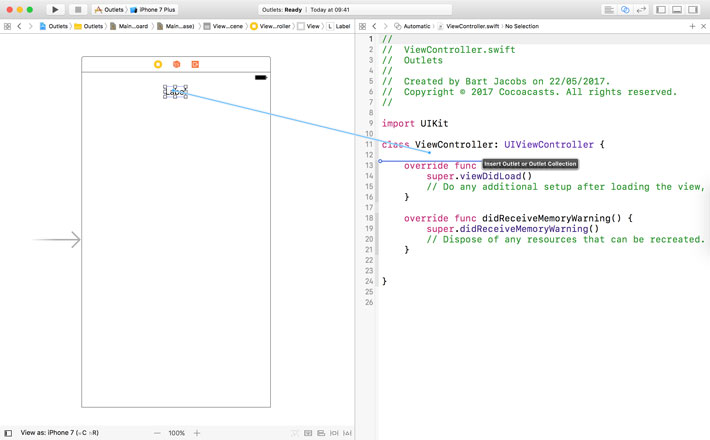
\includegraphics[scale=0.4]{figures/outlets.jpg}
\caption{Para referenciar un elemento de la vista basta con arrastrarlo desde \textit{Interface Builder}.\label{fig:outlets}}
\end{figure}


\paragraph{Actualizar los contenidos de las vistas.} Normalmente suele ocurrir en respuesta a cambios en los datos subyacentes. Podemos vincular un \textit{UIViewController} con un \textit{UIStoryBoard} que es como se conoce al \textit{Interface Builder}. Los elementos de la interfaz se pueden referenciar desde el controlador para modificarlos programáticamente, y se llaman \textit{Outlets}, ver figura~\ref{fig:outlets}.

\begin{figure}[tb]
\centering
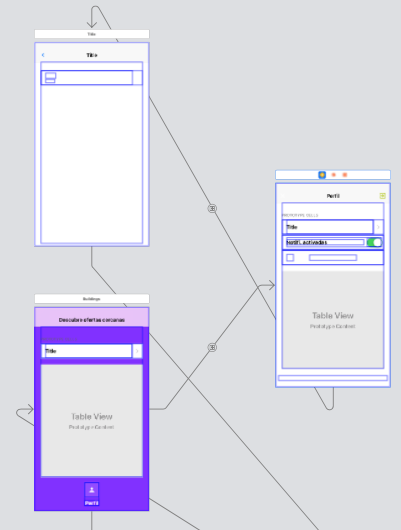
\includegraphics[scale=0.2]{figures/segues.png}
\caption{En \textit{Interface Builder} se definen las relaciones entre controladores (\textit{Segues}). \label{fig:segues}}
\end{figure}

\paragraph{Responder ante las interacciones del usuario con las vistas.} Del mismo modo que vimos en la figura \ref{fig:outlets}, podemos referenciar no sólo los elementos de la interfaz desde el controlador, sino también las distintas acciones que pueden realizar en respuesta a acciones del usuario, y se llaman \textit{Actions}.

\paragraph{Coordinarse con los otros objetos.} Incluyendo otros \textit{UIViewControllers}. Como vimos en el anterior capítulo, se navega de un controlador a otro a mediante el controlador padre o también pueden presentarse los controladores entre ellos. Estas relaciones pueden definirse también en el \textit{Interface Builder}, y se llaman \textit{Segues}, ver figura~\ref{fig:segues}.

























